\section{Evaluation}

\subsection{Experimental Setup}

We evaluate EdgeSched using the deployment configuration described in Section~\ref{sec:implementation}. To make the evaluation criteria explicit, we group the results into five system properties: \textbf{availability}, \textbf{latency degradation}, \textbf{recovery time}, \textbf{throughput overhead}, and \textbf{completion behavior under load}. These categories correspond to the paper's main claims: keeping the resident service reachable, bounding the cost of temporary degradation, restoring high-performance execution predictably, limiting scheduler cost, and remaining operational under mixed workloads and failures.

\textbf{Evaluation Metrics}:
\begin{itemize}
\item \textbf{Availability}: whether the resident service remains usable while the burst workload occupies the GPU
\item \textbf{Latency Degradation}: TTFT (Time To First Token) and visible interruption during migration and coexistence
\item \textbf{Recovery Time}: time required to restore service after workload switching or process failure
\item \textbf{Throughput Overhead}: reduction in aggregate throughput relative to a minimal semaphore-based implementation
\item \textbf{Task Success Rate}: whether submitted tasks complete without observed loss under mixed load and crash scenarios
\end{itemize}

\textbf{Baseline Design Rationale}. We compare EdgeSched against practical alternatives that represent distinct design philosophies rather than arbitrary implementations. \textbf{Cold restart} represents a \emph{restart-based design} that resolves conflicts by killing and reloading the resident workload. \textbf{Operator-managed manual switching} represents an \emph{operator-managed design} in which resource arbitration is pushed outside the runtime and handled through manual model unload/reload steps. \textbf{OS-level paging/LRU-style behavior} represents a \emph{generic memory-management approach} without application-level workload semantics. \textbf{Symmetric migration} represents a \emph{uniform-strategy design} that applies the same stop$\rightarrow$migrate$\rightarrow$resume logic in both directions, without the asymmetric optimization of EdgeSched's Atomic Hot-Swap. For overhead only, we also report a \textbf{raw semaphore-based implementation} as an implementation-cost reference rather than as a full scheduling baseline. Accordingly, the goal of the evaluation is not to show that EdgeSched dominates all generic concurrency mechanisms on synthetic metrics, but to test whether it better matches the service goals of the two-role contention model studied here.

\subsection{Availability and Latency Degradation}

EdgeSched's core capability is enabling a resident, migratable workload and a bursty, GPU-pinned workload to time-share a single 8GB GPU, with the resident workload falling back to system RAM during preemption. In our instantiation, these two workload classes correspond to LLM serving and image generation, respectively.

\subsubsection{Migration Latency and Coexistence}

We measured system behavior during a complete migration cycle: (1) LLM running on GPU, (2) image task preemption (LLM offload to CPU), (3) image task execution, and (4) LLM migration back to GPU. Table~\ref{tab:migration} presents the resource migration performance metrics, and Figure~\ref{fig:migration} visualizes the complete migration timeline showing the asymmetric behavior of downlink (GPU$\rightarrow$CPU) and uplink (CPU$\rightarrow$GPU) paths.

\begin{table}[t]
\centering
\caption{Dynamic Resource Migration Results (N=5)}
\label{tab:migration}
\resizebox{\columnwidth}{!}{%
\begin{tabular}{@{}lcc@{}}
\toprule
\textbf{Metric} & \textbf{EdgeSched} & \textbf{Symmetric Migration} \\
\midrule
LLM GPU TTFT (ms) & 112.9 $\pm$ 12.2 & 87.1 $\pm$ 10.4 \\
CPU TTFT (ms) & 200.0 $\pm$ 19.6 & 209.0 $\pm$ 5.7 \\
Downlink Stutter (ms) & 8774.3 $\pm$ 1768.8 & -- \\
\midrule
Restore Time (ms) & 11237.9 $\pm$ 1226.2 & 5728.3 $\pm$ 148.3 \\
Restore Gap (ms) & $\approx$0 & 1308.9 $\pm$ 2415.0 \\
\midrule
Queue Wait Time (ms) & 10024.8 & -- \\
\bottomrule
\end{tabular}%
}
\end{table}


\begin{figure}[!t]
\centering
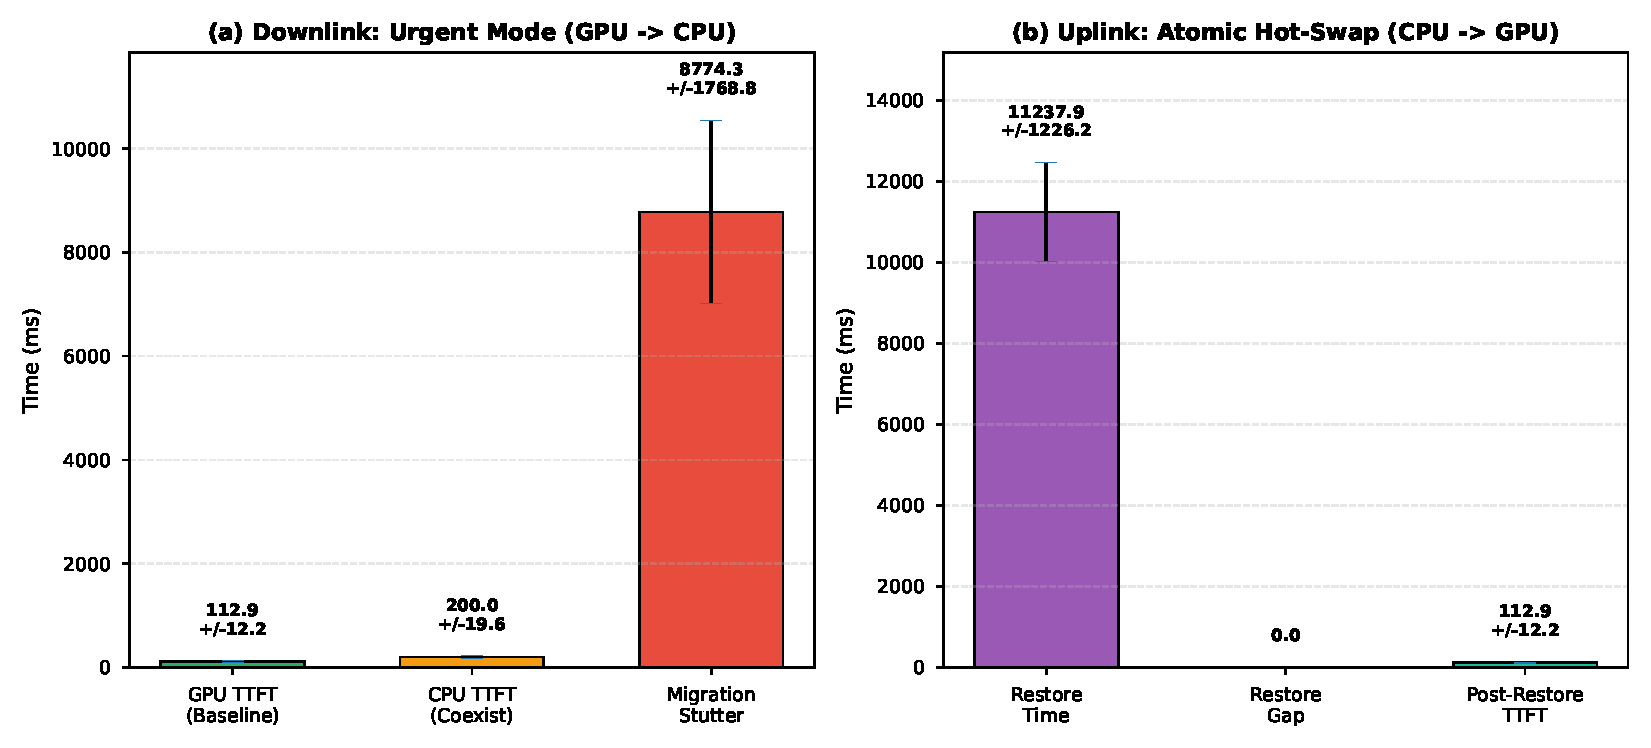
\includegraphics[width=\columnwidth]{figures/01_paper_main/migration/fig_resource_migration.pdf}
\caption{Migration timeline with TTFT measurements. The diagram shows the asymmetric behavior of downlink migration (Urgent Mode) and uplink restoration (Atomic Hot-Swap).}
\label{fig:migration}
\end{figure}

\textbf{Analysis}:
\begin{itemize}
\item \textbf{Availability}: the resident workload remains available during burst-task execution by degrading to CPU service instead of becoming unavailable.
\item \textbf{Low-Interruption Recovery}: User-perceived interruption (Restore Gap) remains near zero in EdgeSched, whereas Symmetric Migration shows a much larger and more variable interruption window of 1308.9 $\pm$ 2415.0 ms. This behavior is consistent with the \textbf{Atomic Hot-Swap} strategy: the CPU instance continues serving requests while the GPU instance preloads in the background.
\item \textbf{Latency Degradation}: In the aggregated migration runs, the logged coexistence TTFT metric is \textbf{200.0 $\pm$ 19.6 ms} for EdgeSched and \textbf{209.0 $\pm$ 5.7 ms} for Symmetric Migration ($N=5$). We treat this logged metric as a scheduler-side indicator rather than a complete characterization of user-perceived latency, and pair it with the real-session trace in Figure~\ref{fig:real_workload}, where CPU-phase request latency ranges from 0.26 to 8.99 s during image execution.
\item \textbf{Migration Cost}: EdgeSched's downlink stutter (\textbf{8774.3 $\pm$ 1768.8 ms}) reflects the cost of Urgent Mode offload. Its restore time (\textbf{11237.9 $\pm$ 1226.2 ms}) is longer than Symmetric Migration's \textbf{5728.3 $\pm$ 148.3 ms}, but that cost is largely hidden behind background preload and near-zero visible cut-over interruption. In other words, EdgeSched optimizes continuity at cut-over rather than raw reload time alone.
\end{itemize}

\subsubsection{Queue Backpressure and Mutual Exclusion}

To verify that availability is preserved under queued burst requests, we submitted concurrent image generation tasks during active LLM sessions.

\begin{itemize}
\item \textbf{Queue Wait Time}: the second image task queued behind the first rather than triggering OOM or overlapping GPU execution
\item \textbf{Behavior}: the system enforced strict GPU mutual exclusion; the second task queued until the first task completed and released resources rather than triggering OOM
\item \textbf{Availability}: throughout image queue processing, the resident LLM service remained responsive on CPU
\end{itemize}

\subsubsection{Real Workload Trace}

Figure~\ref{fig:real_workload} presents the complete timeline of a real interactive session with LLM chat and image generation.

\begin{figure}[H]
\centering
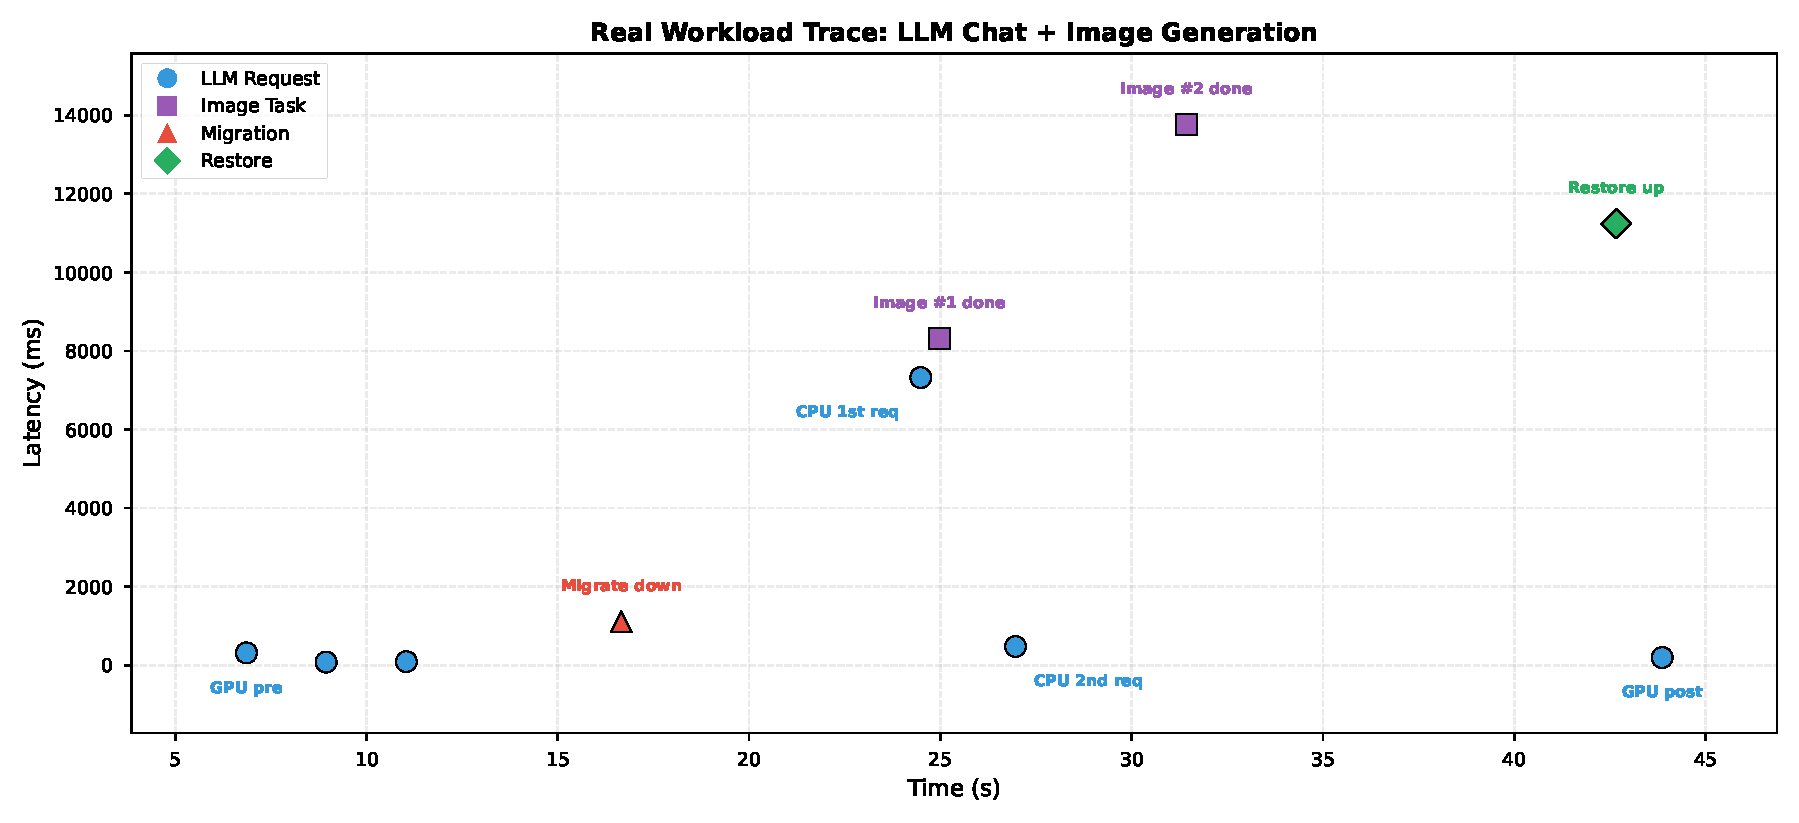
\includegraphics[width=0.96\columnwidth]{figures/02_auxiliary/chart_real_workload_trace.pdf}
\caption{Real workload trace showing TTFT before, during, and after image burst across repeated sessions. GPU TTFT before image: 0.04--0.32s; CPU-phase request latency during image: 0.26--8.99s; restored GPU TTFT: 0.20--2.09s.}
\label{fig:real_workload}
\end{figure}

\textbf{Observations}:
\begin{itemize}
\item \textbf{GPU Phase}: TTFT ranges 0.04--0.32s, demonstrating responsive interaction before burst-task arrival
\item \textbf{Migration}: GPU$\rightarrow$CPU migration takes 1.01--1.13s across the logged sessions
\item \textbf{Coexistence Phase}: CPU-phase request latency ranges from 0.26 to 8.99s during image generation, but the service remains degraded yet available
\item \textbf{Restore}: CPU$\rightarrow$GPU restore takes 10.74--11.53s in the repeated session trace
\item \textbf{Post-Restore}: GPU TTFT returns to 0.20--2.09s after restoration
\end{itemize}

\FloatBarrier

\subsection{Recovery Time}

We evaluate recovery in two forms: \textbf{service recovery} after burst-task completion, and \textbf{failure recovery} after process crash.

\subsubsection{Restart-Based Recovery vs. Atomic Hot-Swap}

We compare the latency of two strategies when switching from image generation back to the resident service: (1) \textbf{Cold Start}, which represents a restart-based design that kills and restarts the resident workload and reloads model weights from disk; and (2) \textbf{Atomic Hot-Swap}, our proposed strategy with KV-cache preservation and instance preloading. Table~\ref{tab:cold_start} presents the comparison across different context sizes.

\begin{table}[H]
\centering
\caption{Recovery Comparison: Cold Restart vs.\ Atomic Hot-Swap}
\label{tab:cold_start}
\resizebox{\columnwidth}{!}{%
\begin{tabular}{@{}lccc@{}}
\toprule
\textbf{Context Size} & \textbf{Cold Restart (ms)} & \textbf{Hot-Swap (ms)} & \textbf{Speedup} \\
\midrule
512 tokens & 3814 $\pm$ 1630 & 972 $\pm$ 123 & 3.9$\times$ \\
1024 tokens & 2477 $\pm$ 205 & 879 $\pm$ 84 & 2.8$\times$ \\
2048 tokens & 3039 $\pm$ 109 & 868 $\pm$ 27 & 3.5$\times$ \\
3072 tokens & 3762 $\pm$ 117 & 948 $\pm$ 102 & 4.0$\times$ \\
\bottomrule
\end{tabular}%
}
\end{table}


\textbf{Key Finding}: Atomic Hot-Swap achieves \textbf{2.8--4.0$\times$} faster recovery than cold restart. Interpreted as a design comparison, this shows that a restart-based approach turns restoration into multi-second service interruption, whereas EdgeSched preserves continuity during background reload and limits visible disruption to the final cut-over.

\subsubsection{Crash Recovery as Lifecycle Robustness}

Beyond migration behavior, we also evaluate whether the scheduler closes task lifecycles correctly under failures. We therefore measure the \textbf{State Backplane}'s recovery performance by injecting random process crashes (SIGKILL) during task execution. Table~\ref{tab:crash_recovery} presents the crash recovery comparison results.

\begin{table}[t]
\centering
\caption{Crash Recovery Comparison}
\label{tab:crash_recovery}
\resizebox{\columnwidth}{!}{%
\begin{tabular}{@{}lccc@{}}
\toprule
\textbf{Metric} & \textbf{Without Backplane} & \textbf{With EdgeSched} & \textbf{Improvement} \\
\midrule
Total Recovery Time (ms) & 7.2 & 44.3 & -- \\
Process Start $\to$ Healthy (ms) & 0.5 & 3.5 & -- \\
Task Recovery Rate & 0\% & \textbf{100\%} & +100\% \\
Tasks Recovered & 0 / 10 & \textbf{10 / 10} & +10 \\
Tasks Lost & 10 & 0 & -100\% \\
\bottomrule
\end{tabular}%
}
\vspace{2pt}
{\small\textit{Note}: Without backplane, process restart is faster but loses all task metadata. With backplane, an additional $\sim$37\,ms buys full semantic recovery.}
\end{table}


\textbf{Analysis}:
\begin{itemize}
\item \textbf{Recovery Time}: with the backplane enabled, the runtime reaches a semantically usable state in 44.3 ms in our measurements, versus 7.2 ms for a process-only restart without task recovery
\item \textbf{Lifecycle Closure}: EdgeSched identifies interrupted "Running" tasks and marks them as recoverable failure states upon restart, avoiding the accumulation of inconsistent task states after crashes
\item \textbf{Recovery Overhead}: startup overhead remains small (about 3 ms), and individual state operations stay below 0.01 ms in our measurements
\end{itemize}

\subsection{Baseline Behavior Under Alternative Designs}

This subsection clarifies how the retained baselines relate to the scheduling claims made in this paper.

Taken together with the restart-based comparison in Table~\ref{tab:cold_start}, the baselines used here cover two practical alternatives in our deployment class: (1) \emph{restart-based restoration}, which releases contention by tearing down and later reloading the resident service; and (2) \emph{OS-managed memory arbitration}, which relies on generic memory-management behavior instead of explicit application-level scheduling. We use these alternatives because they are realistic choices on a single consumer device, even though they do not implement the same service semantics as EdgeSched. The symmetric-migration comparison then isolates a narrower question: whether using different policies for the two migration directions is useful once one accepts the same two-role service model.

We also note an important evaluation limitation. Stronger conceptual references exist in the recent LLM-serving literature, especially phase-disaggregated or interference-aware systems such as Splitwise, P/D-Serve, and Inference without Interference. These systems are closer in spirit to EdgeSched than our practical baselines, but they are not drop-in experimental baselines for this setting because they target server-style LLM serving stacks rather than single-device arbitration between LLM serving and image generation. We therefore use them primarily as positioning references and leave direct reimplementation or adaptation to future work.

\subsubsection{OS-Level Memory Management (Paging/LRU-Style Behavior)}

We evaluate whether OS-level memory management can handle multi-model concurrency without application-level scheduling. This baseline represents a generic memory-management approach \emph{without application-level arbitration}: the system relies on OS-level paging or LRU-style behavior instead of explicit migration control. Because this behavior is sensitive to cache state, we report both cold-start and warm-cache outcomes in Table~\ref{tab:lru}.

\begin{table}[H]
\centering
\caption{OS LRU/Unified Memory Baseline (8GB VRAM)}
\label{tab:lru}
\resizebox{\columnwidth}{!}{%
\begin{tabular}{@{}lcc@{}}
\toprule
\textbf{Scenario} & \textbf{Latency (s)} & \textbf{Status} \\
\midrule
LLM Only (cold start, success runs) & 0.41 $\pm$ 0.00 & Normal \\
Image Only (cold start, success runs) & 4.03 $\pm$ 0.03 & Normal \\
Concurrent LLM (cold start) & Timeout ($>$60s) in 1/5 & Unstable / severe thrashing \\
Concurrent LLM (warm cache) & 9.97 $\pm$ 0.06 & $\sim$59.4$\times$ slower \\
Concurrent Image (warm cache) & 2.02 $\pm$ 0.00 & Completed, but LLM degraded \\
\bottomrule
\end{tabular}%
}
\vspace{2pt}
{\small\textit{Note}: In cold-start runs, OS-level LRU/unified-memory behavior timed out in 1 of 5 iterations. In warm-cache runs, image tasks completed, but concurrent LLM latency remained severely inflated relative to LLM-only execution.}
\end{table}


\textbf{Key Finding}: OS-level paging/LRU-style behavior becomes unusable under our concurrent workload. In the cold-start condition, 1 out of 5 iterations timed out beyond 60s during concurrent execution, indicating that generic paging behavior can fail outright when both large models first contend for VRAM. In the warm-cache condition, the image task completed, but concurrent LLM latency still rose to 9.97 $\pm$ 0.06 s, roughly 59.4$\times$ slower than the warm-cache LLM-only latency of 0.168 $\pm$ 0.002 s. These results show that OS-level memory management is not predictable enough for this setting: cold starts may stall completely, and even warmed runs remain severely degraded.

\subsubsection{Symmetric Migration Baseline}

A natural alternative to EdgeSched's asymmetric design is a \textbf{symmetric migration} strategy that applies the same stop$\rightarrow$migrate$\rightarrow$resume logic in both directions. Under this design, the uplink path (CPU$\rightarrow$GPU) does not use background preloading or atomic hot-swap; instead, it stops the CPU service, loads the GPU model from scratch, and then resumes---the same procedure used in the downlink direction. This baseline is important because it tests whether one unified migration rule can serve both directions well in our setting. Our results indicate that it does not: a procedure optimized for immediate resource release exposes visible restoration interruption, whereas a procedure optimized for seamless restoration would delay resource reclamation. The symmetric baseline therefore helps isolate why EdgeSched's \emph{asymmetry} is useful under the studied constraints, rather than merely cosmetic.

Table~\ref{tab:migration} focuses on the two primary migration designs. In the current aggregated runs, the symmetric migration baseline achieves coexistence availability with CPU TTFT of 209.0 $\pm$ 5.7 ms during burst workload, but its uplink interruption metric is highly variable at 1308.9 $\pm$ 2415.0 ms because service restoration requires stop$\rightarrow$migrate$\rightarrow$resume cut-over. In contrast, EdgeSched's Atomic Hot-Swap keeps visible interruption near zero ($\approx$0 ms) by preloading the GPU instance in the background while the CPU instance continues serving requests.

\textbf{Ablation}. To further isolate the contribution of each optimization direction, we test two ablation variants: (1)~\emph{Fast-down + naive-up}, which uses EdgeSched's urgent offload for the downlink but a naive stop$\rightarrow$migrate$\rightarrow$resume for the uplink; and (2)~\emph{Naive-down + optimized-up}, which uses a naive offload for the downlink but EdgeSched's Atomic Hot-Swap for the uplink. Across these variants, the uplink optimization eliminates user-visible interruption during restoration, while the downlink optimization reduces raw release latency relative to the full EdgeSched path. Read together, these results show a clear trade-off between the two objectives: fast release comes from aggressive downlink handling, whereas continuity comes from delayed cut-over uplink handling. Both optimizations are therefore important to EdgeSched's overall performance profile in the studied deployment setting.

\subsubsection{Operator-Managed Manual Switching Baseline}

We also report an operator-managed manual switching baseline to illustrate the cost of pushing arbitration outside the runtime. Using llama.cpp command-line interface (CLI) tools, the operator manually unloads the resident model, runs the burst workload, and then reloads the resident model.

\textbf{Key Finding}: From manually unloading the resident model, running two image jobs, and reloading the LLM, this path already takes \textbf{18.73s}; the LLM reload alone (1.49s) remains a visible recovery cost after image generation. We treat this result as evidence that external, operator-managed arbitration is practical only as a coarse fallback, not as a substitute for runtime-level scheduling in an interactive local runtime.

\subsection{Throughput Overhead and Task Success Rate}

The remaining results characterize implementation cost and completion behavior under load.

\textbf{Scheduler Overhead}. In a synthetic-load microbenchmark (Mock tasks, $n$=100 per run), EdgeSched showed an approximately 16\% throughput reduction relative to a raw semaphore-based implementation. We report this only as an implementation-cost sanity check rather than as a primary baseline, because such schemes model generic concurrency control rather than mixed-workload resource arbitration. This result should therefore be read as the cost of lifecycle-aware control logic, not as a claim that EdgeSched improves generic synthetic throughput.

\textbf{Stress Characterization}:
\begin{itemize}
\item \textbf{Mock Stress}: In the scheduler-only stress test, the system completed all 2000 mock tasks at 200-way concurrency with no observed failures, and the 10-minute mock soak run processed 5961 tasks with stable RSS around 589 MB (observed range 586--594 MB).
\item \textbf{Realistic Mixed-Workload Stress}: In the 10-minute mixed-workload stress test ($n$=3), EdgeSched completed 65/65 LLM requests and 54/54 image requests, with 54/54 migration and restore cycles succeeding and no crashes observed.
\item \textbf{Latency Under Realistic Load}: Across the realistic stress runs, aggregated LLM TTFT was 0.95 $\pm$ 0.97 s (max 3.37 s), while image latency averaged 16.23 $\pm$ 8.49 s.
\item \textbf{Overhead Interpretation}: The observed ~16\% throughput reduction relative to the raw semaphore approach reflects implementation cost under mock load rather than end-user responsiveness. Under realistic mixed workload, the scheduler maintained full request completion while preserving migration and restore correctness.
\end{itemize}

\begin{figure}[H]
\centering
\IfFileExists{figures/01_paper_main/robustness/fig_stress_test.pdf}{%
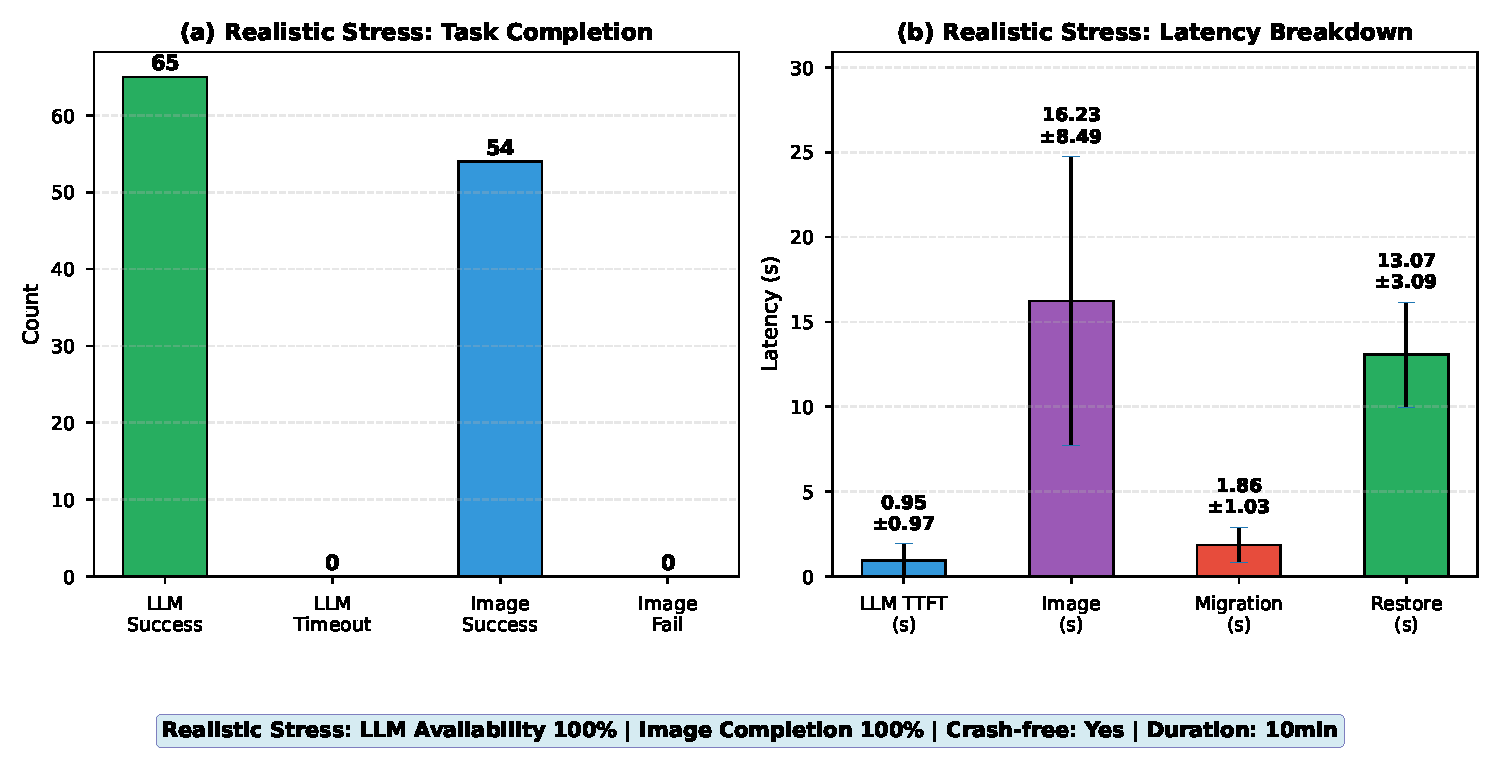
\includegraphics[width=0.96\columnwidth]{figures/01_paper_main/robustness/fig_stress_test.pdf}%
}{%
\fbox{\parbox{0.92\columnwidth}{\centering Stress-test figure unavailable in current workspace build.}}%
}
\caption{Realistic mixed-workload stress results over 10 minutes. The figure summarizes end-to-end completion and latency under repeated LLM/image contention, showing that the system remained crash-free while preserving full request completion in the reported runs.}
\label{fig:stress_test}
\end{figure}


\subsection{Semantic Validation}

We validated specific scheduling semantics that support the workload abstraction and runtime behavior described above.

\begin{enumerate}
\item \textbf{Cancellation}:
\begin{itemize}
\item \textbf{LLM Streaming Cancellation}: The system stops mid-generation at the next cooperative cancellation check.
\item \textbf{Image Queue Cancellation}: Queued tasks are discarded immediately; running tasks continue execution but discard results (soft cancellation).
\end{itemize}

\item \textbf{Priority Inversion}: In our mixed-workload tests, HIGH priority tasks (e.g., user chat) were dispatched ahead of LOW priority tasks (e.g., background summarization) in the queue.
\end{enumerate}

\subsection{Summary}

Taken together, the evaluation shows that EdgeSched is a viable design point for 8GB-VRAM-class consumer devices in our deployment setting. It keeps the resident service reachable during GPU contention, bounds restoration cost through asymmetric migration, recovers task metadata to a semantically usable state in about 44 ms after crashes, sustains full completion in the reported realistic mixed-workload stress runs, and incurs modest mock-workload throughput overhead (~16\%) relative to a minimal semaphore-based implementation.
